\subsection{Data Description}
The training set is 1000 articles, 500 real and 500 fake, of varying length. The development set is 200 articles, 100 fake, 100 real. Articles in development set is truncated to meet the length distribution in Table ~\ref{tab:040dev}. Besides these two sets, we also use a 100 million word corpus of Broadcast News articles as external source for generation of specific feature.
\begin{table}
	\begin{center}
		\begin{tabular}{|c|c|}
		\hline
		\#sentence&\#article\\
		\hline
		1&20\\
		2&10\\
		3&10\\
		4&10\\
		5&10\\
		7&10\\
		10&10\\
		15&10\\
		20&10\\
		\hline
		\end{tabular}
	\end{center}
	\label{tab:040dev}
	\caption{Article length distribution of dev set}
\end{table}
\subsection{Data Preprocessing}
Articles from training set are truncated following the document length distribution in Table ~\ref{tab:040dev}. The number of truncated training articles is 10065. The sentence per article distribution of original training set, truncated training set and development set is shown in Figure ~\ref{fig:040length}.

\begin{figure*}
\centering  
\subfigure[Training set (original)]{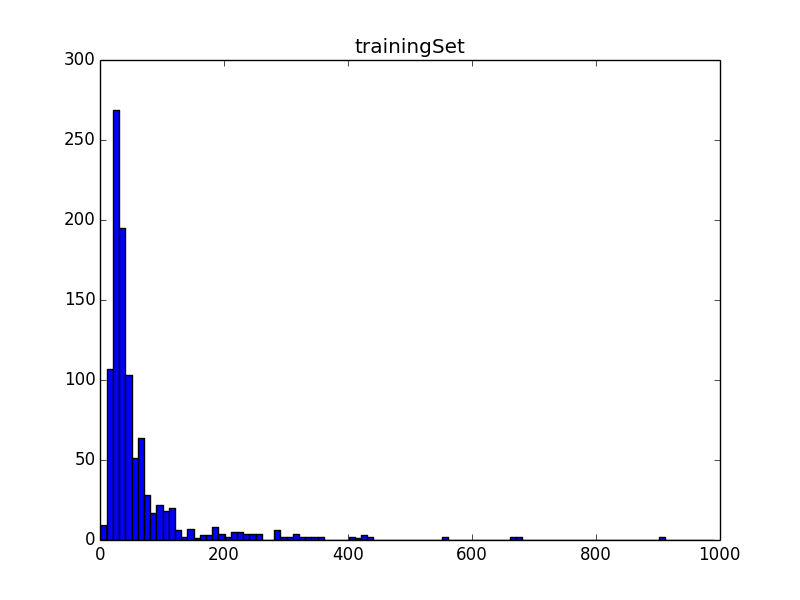
\includegraphics[width=0.33\linewidth]{./FIG/040/trainingdist.png}}\hfill
\subfigure[Training set (truncated)]{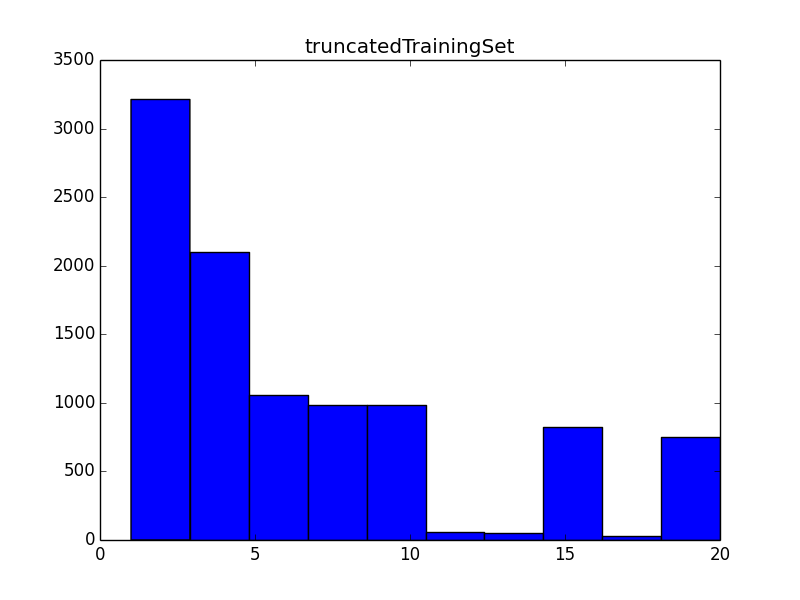
\includegraphics[width=0.33\linewidth]{./FIG/040/trunceddist.png}}\hfill
\subfigure[Dev set]{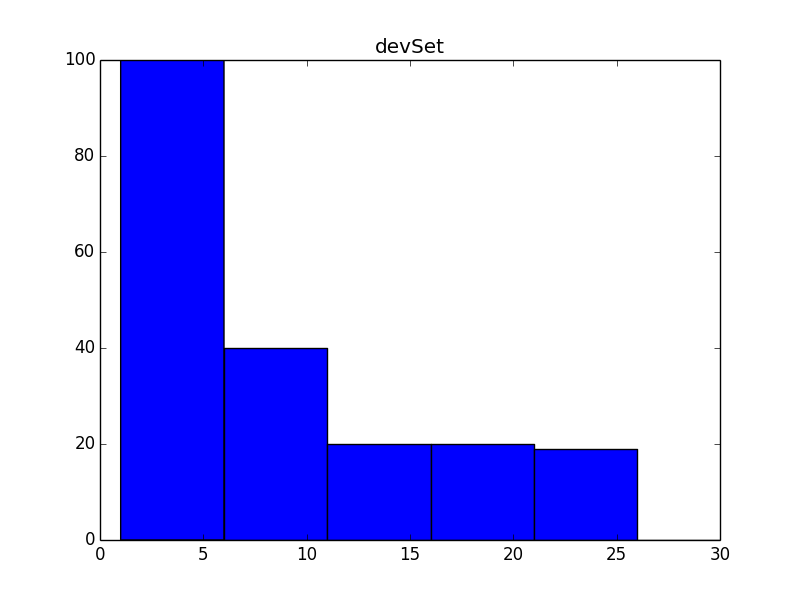
\includegraphics[width=0.33\linewidth]{./FIG/040/devdist.png}}\\

\caption{Article length distribution of different sets}
\label{fig:040length}
\end{figure*}

\subsection{Classifier Choice}
Popular classifiers for binary classification task are chosen as candidates, including KNN, logistic regression, SVM, gradient boosting (xgboost). Testing individual feature on development set and cross validation on training set, xgboost outperforms all the other algorithm by about 5\%. Also it is very fast comparing to SVM. So we choose xgboost as the final classier.

\subsection{Result}